\documentclass{article}
\usepackage{graphicx} % Required for inserting images
\usepackage{subcaption} 
\usepackage{float}
\usepackage{xcolor}
\usepackage{tikz}
\usetikzlibrary{shapes.geometric, arrows.meta, positioning, fit, backgrounds, calc}
\usepackage{pagecolor}
\usepackage{geometry}

\title{Automatic summarization system}
\author{Albert Sirvent Jerez, Enrique Cortés Tárraga and Carlos Sanchis Server}

\date{February 26th, 2026}

\begin{document}

\maketitle

\newpage

\tableofcontents
\newpage

\section{Introduction}

\section{Data}

\section{Architecture}

\begin{figure}[H]
\centering
\resizebox{0.9\textwidth}{!}{%
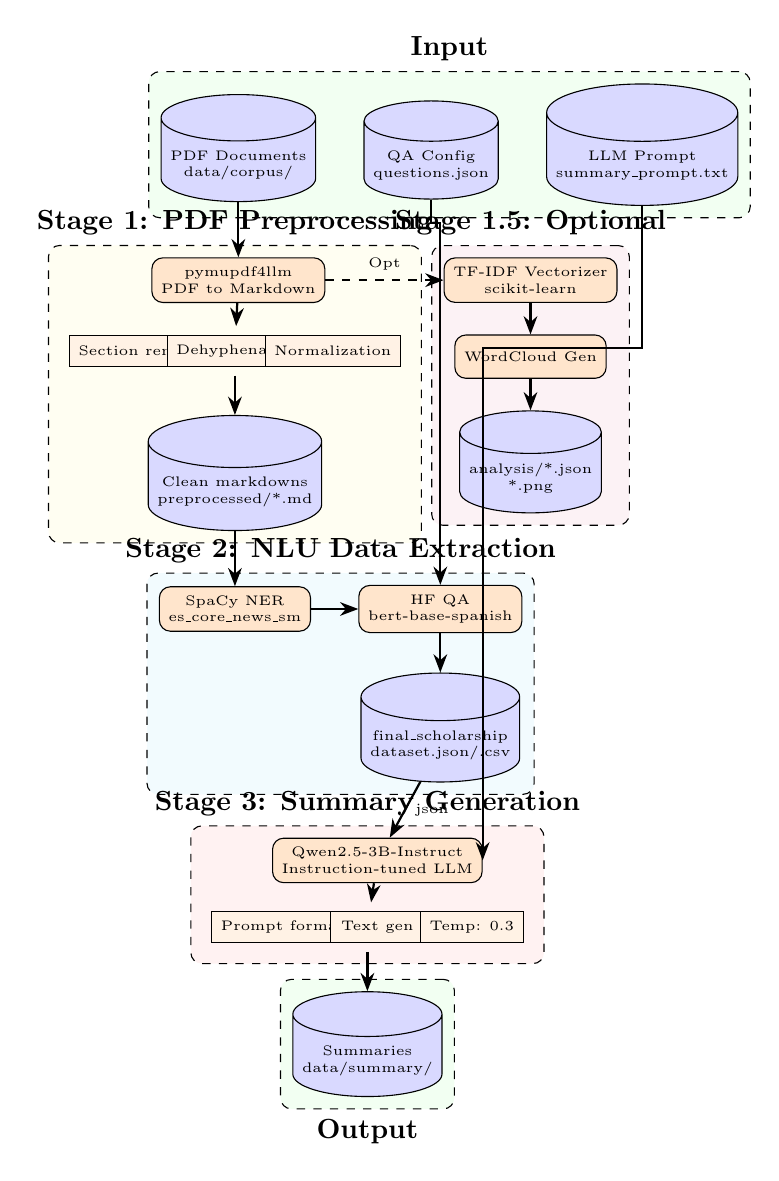
\begin{tikzpicture}[
    node distance=0.35cm and 0.6cm,
    >=Stealth,
    io/.style={cylinder, draw, shape border rotate=90, aspect=0.3, minimum height=0.7cm, minimum width=1.1cm, fill=blue!15, font=\tiny, align=center},
    process/.style={rectangle, draw, rounded corners, minimum height=0.55cm, minimum width=1.5cm, fill=orange!20, font=\tiny, align=center},
    subprocess/.style={rectangle, draw, minimum height=0.4cm, minimum width=1.2cm, fill=orange!10, font=\tiny, align=center},
    subgraph/.style={rectangle, draw, dashed, rounded corners, inner sep=0.15cm, font=\tiny\bfseries},
    arrow/.style={->, thick},
    darrow/.style={->, thick, dashed},
]

% === INPUT SECTION ===
\node[io] (pdf) {PDF Documents\\data/corpus/};
\node[io, right=of pdf] (questions) {QA Config\\questions.json};
\node[io, right=of questions] (prompt) {LLM Prompt\\summary\_prompt.txt};

% Background for Input
\begin{scope}[on background layer]
    \node[subgraph, fill=green!5, fit=(pdf)(questions)(prompt), label=above:\textbf{Input}] (input_bg) {};
\end{scope}

% === STAGE 1: PDF Preprocessing ===
\node[process, below=0.7cm of pdf] (pymupdf) {pymupdf4llm\\PDF to Markdown};

\node[subprocess, below=0.4cm of pymupdf, xshift=-1.2cm] (preprocess1) {Section removal};
\node[subprocess, below=0.4cm of pymupdf] (preprocess2) {Dehyphenation};
\node[subprocess, below=0.4cm of pymupdf, xshift=1.2cm] (preprocess3) {Normalization};

% Background for PREPROCESS
\begin{scope}[on background layer]
    \node[subgraph, fill=yellow!10, fit=(preprocess1)(preprocess2)(preprocess3), inner sep=0.1cm] (preprocess_bg) {};
\end{scope}

\node[io, below=0.5cm of preprocess_bg] (cleanmd) {Clean markdowns\\preprocessed/*.md};

% Background for Stage 1
\begin{scope}[on background layer]
    \node[subgraph, fill=yellow!5, fit=(pymupdf)(preprocess_bg)(cleanmd), label=above:\textbf{Stage 1: PDF Preprocessing}] (stage1_bg) {};
\end{scope}

% === STAGE 1.5: Optional Analysis ===
\node[process, right=1.5cm of pymupdf] (tfidf) {TF-IDF Vectorizer\\scikit-learn};
\node[process, below=0.4cm of tfidf] (wc) {WordCloud Gen};
\node[io, below=0.4cm of wc] (analysisout) {analysis/*.json\\*.png};

% Background for Stage 1.5
\begin{scope}[on background layer]
    \node[subgraph, fill=purple!5, fit=(tfidf)(wc)(analysisout), label=above:\textbf{Stage 1.5: Optional}] (stage15_bg) {};
\end{scope}

% === STAGE 2: NLU Data Extraction ===
\node[process, below=0.7cm of cleanmd] (ner) {SpaCy NER\\es\_core\_news\_sm};
\node[process, right=of ner] (qa) {HF QA\\bert-base-spanish};
\node[io, below=0.5cm of qa] (nluout) {final\_scholarship\\dataset.json/.csv};

% Background for Stage 2
\begin{scope}[on background layer]
    \node[subgraph, fill=cyan!5, fit=(ner)(qa)(nluout), label=above:\textbf{Stage 2: NLU Data Extraction}] (stage2_bg) {};
\end{scope}

% === STAGE 3: Summary Generation ===
\node[process, below=0.7cm of nluout, xshift=-0.8cm] (llm) {Qwen2.5-3B-Instruct\\Instruction-tuned LLM};

\node[subprocess, below=0.35cm of llm, xshift=-1.2cm] (gen1) {Prompt format};
\node[subprocess, below=0.35cm of llm] (gen2) {Text gen};
\node[subprocess, below=0.35cm of llm, xshift=1.2cm] (gen3) {Temp: 0.3};

% Background for GEN
\begin{scope}[on background layer]
    \node[subgraph, fill=red!10, fit=(gen1)(gen2)(gen3), inner sep=0.1cm] (gen_bg) {};
\end{scope}

% Background for Stage 3
\begin{scope}[on background layer]
    \node[subgraph, fill=red!5, fit=(llm)(gen_bg), label=above:\textbf{Stage 3: Summary Generation}] (stage3_bg) {};
\end{scope}

% === OUTPUT SECTION ===
\node[io, below=0.5cm of gen_bg] (summary) {Summaries\\data/summary/};

% Background for Output
\begin{scope}[on background layer]
    \node[subgraph, fill=green!5, fit=(summary), label=below:\textbf{Output}] (output_bg) {};
\end{scope}

% === FLOW CONNECTIONS ===
% Input to Stage 1
\draw[arrow] (pdf) -- (pymupdf);
\draw[arrow] (pymupdf) -- (preprocess_bg);
\draw[arrow] (preprocess_bg) -- (cleanmd);

% Stage 1 to Stage 2
\draw[arrow] (cleanmd) -- (ner);
\draw[arrow] (ner) -- (qa);
\draw[arrow] (qa) -- (nluout);

% Stage 1 to Stage 1.5 (optional)
\draw[darrow] (pymupdf.east) -- node[above, font=\tiny] {Opt} (tfidf.west);
\draw[arrow] (tfidf) -- (wc);
\draw[arrow] (wc) -- (analysisout);

% Questions to QA
\draw[arrow] (questions.south) -- ++(0,-0.3) -| (qa.north);

% Stage 2 to Stage 3
\draw[arrow] (nluout) -- node[right, font=\tiny] {json} (llm);

% Prompt to LLM
\draw[arrow] (prompt.south) -- ++(0,-1.8) -| (llm.east);

% LLM to GEN
\draw[arrow] (llm) -- (gen_bg);

% GEN to Output
\draw[arrow] (gen_bg) -- (summary);

\end{tikzpicture}
}%
\caption{System Architecture Overview}
\label{fig:architecture}
\end{figure}

\section{Evaluation}

In this stage is where we use the information extracted in the previous stage to generate a summary of each document, trying to capture all the information possible and focus it in a clear way.
During the development, we decided to separate this stage from the initial one, so to be able to run it independently, as the information extraction is a very time-consuming process.

\subsection{Model Election}

The first step of this stage is to choose the language generation model that we will use to generate the summaries. 
We were thinking on using Ollama to generate the summaries but we tried to keep everything "within" Hugging-Face.
Our first choices were focused on lightweight models only trained in spanish, these were the ones we tested (with the issues we found):

\begin{itemize}

\item \textbf{SEBIS/legal\_t5\_small\_summ\_es} \\
\textit{Objective:} Small T5 model fine-tuned for legal text summarization in Spanish. \\
\textit{Issue encountered:} Not instruction-following and unable to reliably interpret structured JSON inputs.

\item \textbf{mrm8488/bert2bert\_shared-spanish-finetuned-summarization} \\
\textit{Objective:} Encoder-decoder model based on BETO fine-tuned for Spanish news summarization (MLSUM). \\
\textit{Issue encountered:} Technical instability on macOS (meta tensor errors) and poor adaptation to structured dictionary inputs.

\item \textbf{Narrativa/bsc\_roberta2roberta\_shared-spanish-finetuned-mlsum-summarization} \\
\textit{Objective:} RoBERTa2RoBERTa model trained for abstractive news summarization in Spanish. \\
\textit{Issue encountered:} Designed for continuous narrative text rather than structured JSON data.

\end{itemize}

After having little success with the previous models, we decided to try multilingual models (with spanish support) and we also removed our requirement to have it lightweight.
We thought on using instruction-tuned, as they work better for transforming structured JSON inputs into coherent narrative text (they are explicitly trained to interpret task-specific instructions rather than summarize).

\begin{itemize}

\item \textbf{google/flan-t5-small} \\
\textit{Objective:} Instruction-tuned multilingual model capable of following prompts and generating Spanish text. \\
\textit{Issue encountered:} Limited coherence and coverage when handling long or complex JSON inputs.

\item \textbf{Qwen/Qwen2.5-3B-Instruct (Selected Model)} \\
\textit{Objective:} Multilingual instruction-following model optimized for structured input understanding and coherent text generation. \\
\textit{Issue encountered:} Higher computational requirements compared to smaller summarization models.

\end{itemize}

Finally, we decided to use the Qwen2.5-3B-Instruct model, as it was the one that generated the best summaries and was able to understand better the structured input without being "too big" or too slow.

\subsection{Prompt Used}

The generation stage relies on a single instruction-based prompt designed to transform the structured JSON output into a fluent, article-style text in Spanish. The model is explicitly instructed to behave as a public policy writer and to produce a coherent narrative description of the scholarship without mentioning the JSON structure or using bullet points. 

The prompt enforces coverage of key elements (academic year, target studies, financial components, income thresholds, deadlines, and special conditions) while explicitly prohibiting hallucinations or the addition of information not present in the input. This design ensures that the generated text remains faithful to the extracted structured data while adopting a natural journalistic style.

The exact prompt used in the system is shown below:

\begin{verbatim}
Eres un redactor especializado en convocatorias públicas.
A partir del siguiente JSON, redacta un texto informativo en español 
como si fuera un artículo explicando en qué consiste la beca.

El texto debe:
- Explicar el curso académico al que corresponde.
- Indicar a qué enseñanzas o estudios se dirige.
- Describir las cuantías principales (renta, residencia, básica, 
  variable, excelencia si existe).
- Mencionar los umbrales de renta si aparecen.
- Explicar los plazos de solicitud.
- Incluir condiciones especiales (discapacidad, insularidad, víctimas) 
  si están presentes.

No inventes información.
No añadas datos que no estén en el JSON.
No menciones el JSON ni uses formato estructurado.
Redacta un texto fluido de entre 8 y 15 líneas.

JSON:
{json_text}

Artículo:
\end{verbatim}

\subsection{Model Evaluation}

The generation stage was evaluated using the structured JSON dataset as input and comparing the produced summaries across all academic years. 
The main differences observed between the tested models were related to their ability to interpret structured JSON inputs and transform them into coherent narrative text, as well as their stability in a local environment.

Finally, the selected model (Qwen2.5-3B-Instruct) demonstrated solid instruction-following capabilities and good narrative quality, the only caveat was the generation length as we has several issues with truncation when the generated text was too long, so we had to adjust the generation parameters to ensure that the output remained within a reasonable length while still capturing all relevant information.

The main observations are summarized below.

\subsubsection{Strengths}

\begin{itemize}
    \item Produces fluent, coherent article-style texts in Spanish.
    \item Correctly introduces the academic year and overall purpose of the scholarship.
    \item Integrates multiple financial components (income-linked, residence-linked, basic and variable amounts) into a unified narrative.
    \item Includes excellence-related bonuses and special conditions (e.g., disability increments) when clearly present in the JSON.
    \item Transforms structured numerical values into readable natural language without relying on bullet-point formatting.
    \item Maintains consistent tone and structure across all academic years.
\end{itemize}

\subsubsection{Limitations and Areas for Improvement}

\begin{itemize}
    \item Propagates inconsistencies present in the extracted JSON (e.g., conflicting deadlines or imprecise values).
    \item Occasionally simplifies or slightly misinterprets categorical fields when the input is ambiguous.
    \item Does not perform logical validation across fields (e.g., checking temporal coherence between academic year and deadlines).
    \item Output length must be carefully controlled to avoid truncation in longer summaries.
\end{itemize}

\section{Conclusion}

......

In the generation stage, model selection proved crucial for producing coherent and faithful summaries. Lightweight Spanish summarization models were not suitable for structured JSON inputs, whereas instruction-tuned multilingual models performed significantly better.

The selected model, Qwen2.5-3B-Instruct, achieved a good balance between narrative quality and structured input understanding. However, generation quality remains strongly dependent on the accuracy of the information extraction stage, as inconsistencies in the extracted data are directly reflected in the final summaries.

Overall, the generation stage successfully produced coherent and informative texts aligned with the structured input.

\end{document}
